%%%%%%%%%%%%%%%%%%%%%%%%%%%%%%%%%%%%%%%%%
% Structured General Purpose Assignment
% LaTeX Template
%
% This template has been downloaded from:
% http://www.latextemplates.com
%
% Original author:
% Ted Pavlic (http://www.tedpavlic.com)
%
% Note:
% The \lipsum[#] commands throughout this template generate dummy text
% to fill the template out. These commands should all be removed when 
% writing assignment content.
%
%%%%%%%%%%%%%%%%%%%%%%%%%%%%%%%%%%%%%%%%%

%----------------------------------------------------------------------------------------
%	PACKAGES AND OTHER DOCUMENT CONFIGURATIONS
%----------------------------------------------------------------------------------------

\documentclass{article}

\usepackage{fancyhdr} % Required for custom headers
\usepackage{lastpage} % Required to determine the last page for the footer
\usepackage{extramarks} % Required for headers and footers
\usepackage{graphicx} % Required to insert images
\usepackage{lipsum} % Used for inserting dummy 'Lorem ipsum' text into the template
\usepackage{longtable}

% Margins
\topmargin=-0.45in
\evensidemargin=0in
\oddsidemargin=0in
\textwidth=6.5in
\textheight=9.0in
\headsep=0.25in 

\linespread{1.1} % Line spacing

% Set up the header and footer
\pagestyle{fancy}
\lhead{Nelson \& Sergii} % Top left header
\chead{\hmwkClass: \hmwkTitle} % Top center header
%\chead{\hmwkClass\ (\hmwkClassInstructor\ \hmwkClassTime): \hmwkTitle} % Top center header
\rhead{\firstxmark} % Top right header
\lfoot{\lastxmark} % Bottom left footer
\cfoot{} % Bottom center footer
\rfoot{Page\ \thepage\ of\ \pageref{LastPage}} % Bottom right footer
\renewcommand\headrulewidth{0.4pt} % Size of the header rule
\renewcommand\footrulewidth{0.4pt} % Size of the footer rule

\setlength\parindent{0pt} % Removes all indentation from paragraphs

%----------------------------------------------------------------------------------------
%	DOCUMENT STRUCTURE COMMANDS
%	Skip this unless you know what you're doing
%----------------------------------------------------------------------------------------

% Header and footer for when a page split occurs within a problem environment
\newcommand{\enterProblemHeader}[1]{
\nobreak\extramarks{#1}{#1 continued on next page\ldots}\nobreak
\nobreak\extramarks{#1 (continued)}{#1 continued on next page\ldots}\nobreak
}

% Header and footer for when a page split occurs between problem environments
\newcommand{\exitProblemHeader}[1]{
\nobreak\extramarks{#1 (continued)}{#1 continued on next page\ldots}\nobreak
\nobreak\extramarks{#1}{}\nobreak
}

\setcounter{secnumdepth}{0} % Removes default section numbers
\newcounter{homeworkProblemCounter} % Creates a counter to keep track of the number of problems

\newcommand{\homeworkProblemName}{}
\newenvironment{homeworkProblem}[1][Problem \arabic{homeworkProblemCounter}]{ % Makes a new environment called homeworkProblem which takes 1 argument (custom name) but the default is "Problem #"
\stepcounter{homeworkProblemCounter} % Increase counter for number of problems
\renewcommand{\homeworkProblemName}{#1} % Assign \homeworkProblemName the name of the problem
\section{\homeworkProblemName} % Make a section in the document with the custom problem count
\enterProblemHeader{\homeworkProblemName} % Header and footer within the environment
}{
\exitProblemHeader{\homeworkProblemName} % Header and footer after the environment
}

\newcommand{\problemAnswer}[1]{ % Defines the problem answer command with the content as the only argument
%\noindent\framebox[\columnwidth][c]{\begin{minipage}{0.98\columnwidth}#1\end{minipage}} % Makes the box around the problem answer and puts the content inside
}

\newcommand{\homeworkSectionName}{}
\newenvironment{homeworkSection}[1]{ % New environment for sections within homework problems, takes 1 argument - the name of the section
\renewcommand{\homeworkSectionName}{#1} % Assign \homeworkSectionName to the name of the section from the environment argument
\subsection{\homeworkSectionName} % Make a subsection with the custom name of the subsection
\enterProblemHeader{\homeworkProblemName\ [\homeworkSectionName]} % Header and footer within the environment
}{
\enterProblemHeader{\homeworkProblemName} % Header and footer after the environment
}
   
%----------------------------------------------------------------------------------------
%	NAME AND CLASS SECTION
%----------------------------------------------------------------------------------------

\newcommand{\hmwkTitle}{Final Project} % Assignment title
\newcommand{\hmwkDueDate}{Friday,\ September\ 19,\ 2017} % Due date
\newcommand{\hmwkClass}{ANLY\ 515-50-2017} % Course/class
\newcommand{\hmwkClassTime}{7:00pm} % Class/lecture time
\newcommand{\hmwkClassInstructor}{Dr. Martin A. Negron} % Teacher/lecturer
\newcommand{\hmwkAuthorName}{Nelson Corrocher} % Your name
\newcommand{\hmwkAuthorNameB}{Sergii Savchuk} % Your name

%----------------------------------------------------------------------------------------
%	TITLE PAGE
%----------------------------------------------------------------------------------------

\title{
\vspace{2in}
\textmd{\textbf{\hmwkClass:\ \hmwkTitle}}\\
\normalsize\vspace{0.1in}\small{Due\ on\ \hmwkDueDate}\\
\vspace{0.1in}\large{\textit{\hmwkClassInstructor\ \hmwkClassTime}}
\vspace{3in}
}

\author{\textbf{\hmwkAuthorName} \\
		\textbf{\hmwkAuthorNameB}}
\date{} % Insert date here if you want it to appear below your name

%----------------------------------------------------------------------------------------

\begin{document}

\maketitle

%----------------------------------------------------------------------------------------
%	TABLE OF CONTENTS
%----------------------------------------------------------------------------------------

%\setcounter{tocdepth}{1} % Uncomment this line if you don't want subsections listed in the ToC

\newpage
\tableofcontents
\newpage

%----------------------------------------------------------------------------------------
%	TOPIC SELECTION
%----------------------------------------------------------------------------------------

% To have just one problem per page, simply put a \clearpage after each problem

\begin{homeworkProblem}[TOPIC SELECTION]
\paragraph{}The movie we selected is Rounders(1998). It is about a Poker player that dreams about winning the World Series of Poker (WSOP) but lose his entire bankroll in an "unlucky" hand at the beginning scene. We chose these movie firstly because its representation of poker games is considered sober and very realistic (no straight-flush vs quads or lower quads vs high quads, no unrealistic bluffs). Additionally, most of the events used in the Bayes network are based of poker hand probabilities and their marginal probability is well known, reducing the need of guesswork.
\paragraph{}Most of the risks in this movie involve the player playing against adversaries and the adversary's behavior during the match influencing the decisions of the protagonist, in addition to external factors mitigating the probabilities like players cheating, bad judgment, gangsters pressuring the player, etc.
With this model we could analyze two questions about this movie:
\begin{itemize}
	\item{In the beginning of the movie, was it good judgment when Mike went all-in against Ted KGB after the "river" (last card) was flopped in the table?}
	\item{\textbf{UPDATED:} In such situation, what would have been the best move for Mike to do instead?}
\end{itemize}
\paragraph{}Most of the data from this analysis can be collected from the movie itself since poker hand probabilities are well understood. Some guesswork may be involved when calculating the probabilities of some subjective events to happen or influence outcomes.
\end{homeworkProblem}

\begin{homeworkProblem}[ANALYSIS]
	\paragraph{}\textbf{Introduction:}
	\paragraph{}As mentioned above, the movie is about Mike, a professional poker player who wanted to play at the World Series of Poker (WSOP), until he lost all his money in a single hand to another professional gambler, Teddy KGB. The remaining of the movie focus on his recovery. This movie was selected for having excellent examples of practical application of Bayesian networks and because the marginal probabilities of poker hand won't involve much guesswork. 
	\paragraph{}In our analysis, we are going to focus on poker hand played at the beginning of the movie, the one in which Mike lost his entire bankroll of \$30,000. We also need to establish some game theory assumptions to proceed:
	\begin{itemize}
		\item Both players are rational and trying to maximize their profit. (Game theory assumption)
		\item Both players are very experienced, both at professional level (Don't make dumb plays)
		\item No cheating involved (on that hand)
	\end{itemize}
	The probabilities calculated below came from Poker Hand simulators and the theory behind it, from the great poker book from David Sklansky and Ed Miller, No Limit Hold'em. We also used Nelson's experience as a poker player.
	\clearpage
	\paragraph{}\textbf{Process and Model:}
	\paragraph{}The first step was to watch again the movie and take notes about cards, positions, bettings and pot size. Description of the match settings:
	\begin{itemize}
		\item Four players playing
		\item Mike at dealer's position and Teddy KGB at big blind's
		\item Blinds of \$50-\$100
		\item Mike had a stack of about \$45,000 (started the game with \$30,000)
	\end{itemize}
	Below we detail how that round was played:
	\begin{itemize}
	\item Mike received A9 clubs-suited
	\item First players folds
	\item Mike raises the pre-flop bet to \$500
	\item Second player on small blind folds
	\item Teddy calls it (\textbf{IMPORTANT EVENT}). Pot is now \$1,050
	\item Three first community cards (Flop) are showed: A-Spades, 9-Spades, 8-Clubs. Now Mike has top two-pair hand
	\item Teddy KGB checks (uncommon play for AA which and while a noteworthy, don't convey any significant information for the model)
	\item Mike bet \$2,000 on a pot of \$1,050. Pot is now \$3,050
	\item Teddy calls (\textbf{IMPORTANT EVENT}). Pot is now \$5,050
	\item Turn (4th community card) showed: 9-Hearts. Mike now has a 9s Full of Aces.
	\item Both players check
	\item River (5th community card) showed: 3-Spades.
	\item Teddy bets \$15,000 on a \$5,050 pot (\textbf{IMPORTANT EVENT}).
	\item Mike goes all-in with 15,000 + 33,000 for a total pot of \$68,050.
	\item Teddy calls and shows two Aces, making a Aces of Nines, beating him.
	\end{itemize}
	\paragraph{}With the facts shown above, let's start with the model. In the river, Mike had Nines Full of Aces, which could only be beaten by Aces full of Nines (pocket Aces). If this information in inserted in any on-line poker calculator, it is going to show that such hand has a chance of winning of \textbf{99.70\%}. This is our marginal probability of wining and our first step:
	\begin{center}
		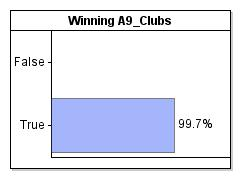
\includegraphics{Image1.jpg}
	\end{center}
	\paragraph{}Moving on, since the only hand that could beat Mike's game was an AA, making the Aces full of Nines, let's rephrase the problem: What is the chance that Teddy had pocket aces? Obviously, the marginal probability is the same but FALSE instead of TRUE (Wining is 99.7\% TRUE while having AA is 99.7\% FALSE). With this let's start calculating the conditional probabilities on the three events mentioned above.
	\paragraph{}One rule of thumb used by professional players is to play only the top 25\% hands so we assume that when Teddy called the pre-flop bet. We order the pre-flop hands by expected chance of winning and there are many tables in books and in the internet that shows this listing. From 169 possible hands, he now was reduced to 41 hands (excluding the AA, a separate event). In terms of our model, if he has pocket aces, he will play 100\% of the time. If he doesn't, he would play only about 25\% of the time, as below:
	\begin{center}
		\begin{tabular}{||c c c||} 
			\hline
			\textbf{Has pocket-Aces} & \textbf{True} & \textbf{False} \\ [0.5ex] 
			\hline
			PreFlopCall-True & 1.00 & 0.25 \\ 
			\hline
			PreFlopCall-False & 0.00 & 0.75 \\
			\hline
		\end{tabular}
	\end{center}
	\paragraph{}The second important event is when Teddy called overbet made by Mike. When Mike bet \$2,000 on a \$1,050 pot table, he got Teddy in a situation in which he would call only if he had chances higher than \$3,050-to-\$2,000 against (or 1.525-to-1). In probability terms, it means that for Teddy to call he would need to believe he had a chance better than \textbf{39.6\%} to win. Without getting too much into the weeds here, with such flop, he would call only if he had a flush-draw (situation in which he is one suit away from making a flush), a set (trips made with pocket-pair) or two pairs. Looking at the hands left and matching the ones that could possibly match this criteria, we get 33 of 41, giving us a probability of cold calling 100\% of the time if he has aces, and only 82.9\% if he doesn't. This information is conveyed by the table below:
	\begin{center}
		\begin{tabular}{||c c c||} 
			\hline
			\textbf{Has pocket-Aces} & \textbf{True} & \textbf{False} \\ [0.5ex] 
			\hline
			FlopCall-True & 1.00 & 0.830 \\ 
			\hline
			FlopCall-False & 0.00 & 0.170 \\
			\hline
		\end{tabular}
	\end{center}
	\paragraph{}The third important event is when Teddy bets \$15,000 after the River, on a pot of \$5,050. This gives a ratio of 5,050-to-15,000 against, thus calling it requires would require a belief of the hand winning in 74.8\% of the time. Converting this to poker hands, we can eliminate any lower flushes and any two pair. Either he would have a pocket-pair set (making a full house) or the highest flush. This reduces the total hands to 6 of 33. This time, however, it is not 100\% chance he would bet having AA because he could be aiming for Mike to bet so him could raise. A fair assumption here is something closer to 50\% to avoid scaring the opponent and risking losing the jackpot. Without AA, the chance of such huge bet would go only to 20.6\%, as shown in the table below:
		\begin{center}
		\begin{tabular}{||c c c||} 
			\hline
			\textbf{Has pocket-Aces} & \textbf{True} & \textbf{False} \\ [0.5ex] 
			\hline
			Bet-True & 0.50 & 0.206 \\ 
			\hline
			Bet-False & 0.50 & 0.794 \\
			\hline
		\end{tabular}
	\end{center}
	\paragraph{}After putting all of this together in AgenaRisk, setting the three events to true and running the model, we can see how unbelievably high the chance of the opponent having pocket-aces increases from \textbf{0.003\%} to \textbf{92.12\%}. Even when playing with different scenarios and assuming other types of behaviors, like aggressive/passive, tight/loose, etc., we could only reduce the probability to \textbf{77.17\%} lowest.
	\paragraph{}Below we provide a screen-shot of the model made with AgenaRisk:
	\begin{center}
			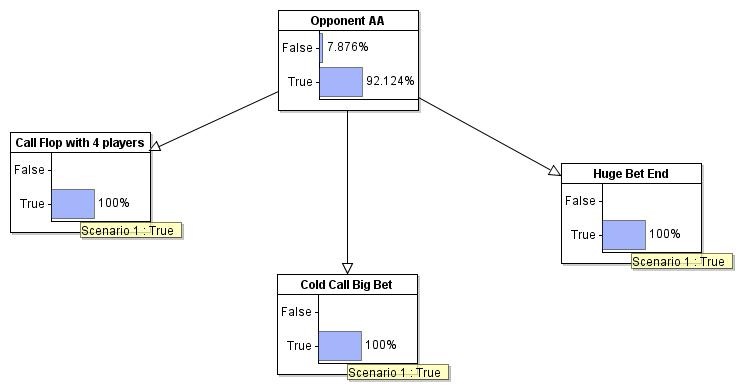
\includegraphics[width=\textwidth,keepaspectratio]{Main_Scenario.jpg} % Example image
	\end{center}
	\paragraph{}\textbf{NOTE: }Even though this model seems to have three independent events, this is not the case. The right event is dependent on the middle, left and root events; the middle event is dependent on the left and root events. Since we were interested only in the case the three events happen simultaneously, we incorporated in each event the conditional probabilities of dependent events. Example: The first event happens in 25\% the time. When the second event happens, its new information is added over the remaining 25\% of the hands from the first event. Thus this model only works because the observations on the three events are set to true. You can't select observation of true only in the second event, for example, as that would make the outcome incorrect.
	\paragraph{}Now, with this model and using some odds math we can show how bad was the decision that Mike made. Let's first calculate the payoff. 20,050-to-15,000 against (1.336-to-1 ratio). For him to profitably call, he would need chance of winning greater than 42.8\%. As we saw in the model, his chance of winning in the best case, would be only 17.6\%. Not just he called it, but he also raised it, making the effective payoff of 20,050 to 48,000 (0.4178-to-1), which would require a probability of winning of 70.53\% to make it profitable. 
	\paragraph{}Now for the second question, could Mike have done something better? Yes. In that round, he made two mistakes: The first one, was to play the game with his entire bankroll. Even if his chances were different and favorable (positive utility), he could get unlucky in one hand, losing everything, even if playing well. No matter how positive your utility, bankruptcy will always end your chances of recovering in an unlucky event. No probability study will help in this situation.
	\paragraph{}The second mistake was his play after the river. There was absolutely no benefit for him to go all-in. This is one of the cases that he had everything to lose and nothing to win: If Teddy didn't have the nuts (biggest possible game in a hand), he would have fold, paying only in the case he had the nuts. The best thing he could have done was to fold the last hand. Now, realistically speaking, folding in such situation would be very difficult and uncommon, even for professionals. Calling it would be the realistic approach; he would still have money to continue playing and recovering his losses (in fact, he would have more money than when he sat on the table to play so he was still in a favorable position). 
	\paragraph{}In summary, any other action would have been a better option than raising the river. Just calling would be the realistic play for good players in such situation. The best play, though unlikely, would be to fold it.

	\paragraph{}For curiosity, we also created two other scenarios. One if Teddy would play loosely (playing a wide number of hands that otherwise wouldn't be playable) and betting on the case he had a high flush. Below:
	\begin{center}
		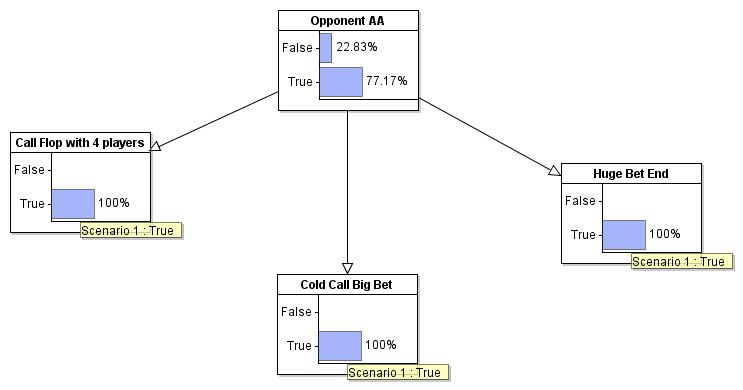
\includegraphics[width=\textwidth,keepaspectratio]{Scenario_2.jpg}
	\end{center}
	\clearpage
	\paragraph{}Finally, we also tried a more mathematical calculation (but somewhat unfeasible for a real world play), in which we calculated all possible hand combinations for the each of game hands in the main Scenario (example: since there was already one A in Mikes and another A in the table, there was only one possibility for Teddy to have AA; a KK would have 6 combinations because no K was into play yet) the player could have. Total combinations of 1326. 
	\begin{center}
		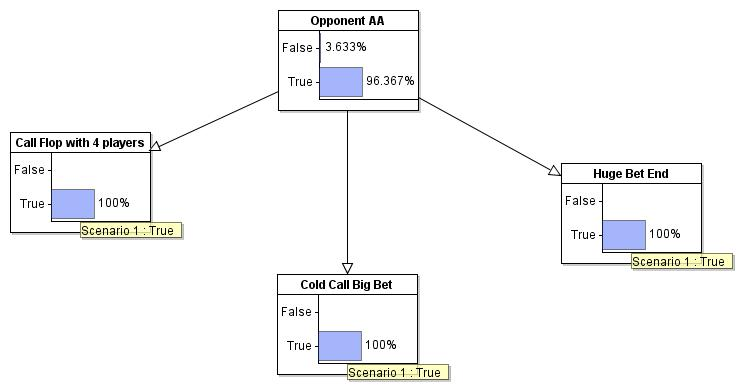
\includegraphics[width=\textwidth,keepaspectratio]{Scenario_3.jpg}
	\end{center}		
\end{homeworkProblem}

\begin{homeworkProblem}[APPENDIX]
\end{homeworkProblem}
		\begin{longtable}{l l l l l l}	
			\caption{Poker-Hands and probabilities of winning against two players}\\
			\hline\\
			&  & First call on pre-flop & Call on flop & Big bet on River \\
			Cards & 2 plyrs & Combinations & Hands Left & Hands Left \\
			88 & 69.10\% & 6 & 3 & 3 \\
			A9o & 60.90\% & 12 & 3 & 3 \\
			A9s & 63.00\% & 4 & 2 & 2 \\
			AA & 85.30\% & 6 & 1 & 1 \\
			99 & 72.10\% & 6 & 1 & 1 \\
			A8o & 60.10\% & 12 & 6 & 0 \\
			A7s & 61.10\% & 4 & 3 & 0 \\
			QTs & 59.50\% & 4 & 3 & 0 \\
			K8s & 58.50\% & 4 & 3 & 0 \\
			AKs & 67.00\% & 4 & 2 & 0 \\
			AQs & 66.10\% & 4 & 2 & 0 \\
			KQs & 63.40\% & 4 & 2 & 0 \\
			KJs & 62.60\% & 4 & 2 & 0 \\
			A8s & 62.10\% & 4 & 2 & 0 \\
			KTs & 61.90\% & 4 & 2 & 0 \\
			QJs & 60.30\% & 4 & 2 & 0 \\
			AJs & 65.40\% & 4 & 1 & 0 \\
			ATs & 64.70\% & 4 & 1 & 0 \\
			KK & 82.40\% & 6 & 0 & 0 \\
			QQ & 79.90\% & 6 & 0 & 0 \\
			JJ & 77.50\% & 6 & 0 & 0 \\
			TT & 75.10\% & 6 & 0 & 0 \\
			77 & 66.20\% & 6 & 0 & 0 \\
			AKo & 65.40\% & 12 & 0 & 0 \\
			AQo & 64.50\% & 12 & 0 & 0 \\
			AJo & 63.60\% & 12 & 0 & 0 \\
			66 & 63.30\% & 6 & 0 & 0 \\
			ATo & 62.90\% & 12 & 0 & 0 \\
			KQo & 61.40\% & 12 & 0 & 0 \\
			KJo & 60.60\% & 12 & 0 & 0 \\
			55 & 60.30\% & 6 & 0 & 0 \\
			A6s & 60.00\% & 4 & 0 & 0 \\
			K9s & 60.00\% & 4 & 0 & 0 \\
			A5s & 59.90\% & 4 & 0 & 0 \\
			KTo & 59.90\% & 12 & 0 & 0 \\
			A7o & 59.10\% & 12 & 0 & 0 \\
			A4s & 58.90\% & 4 & 0 & 0 \\
			QJo & 58.20\% & 12 & 0 & 0 \\
			A3s & 58.00\% & 4 & 0 & 0 \\
			K9o & 58.00\% & 12 & 0 & 0 \\
			Q9s & 57.90\% & 4 & 0 & 0 \\
			A6o & 57.80\% & 12 & 0 & 0 \\
		&  &  &  &  \\
			NOTES &  & Top 25\% of hands & Two-pairs, trips or flush-draws & Full-house only
		\end{longtable}
	
	\begin{homeworkProblem}[BIBLIOGRAPHY]
		\paragraph{}Sklansky, D. and Miller, E. (2007). No limit hold'em theory and practice. Henderson, Nev.: Two Plus Two Pub.\\
		\paragraph{}Cardplayer.com. (2017). Texas Hold'em Odds Calculator. [online] Available at: http://www.cardplayer.com/poker-tools/odds-calculator/texas-holdem [Accessed 14 Sep. 2017].\\
		\paragraph{}Natesholdem.com. (2017). Flop Odds, Probability, Texas Holdem Poker, Tips, Odds, Tells. [online] Available at: http://www.natesholdem.com/pre-flop-odds.php [Accessed 14 Sep. 2017].
	\end{homeworkProblem}
\end{document}
